\chapter{Neural Networks and Deep Learning}
\section*{Learning Objectives}
\begin{itemize}
  \item Understand the major technology trends driving Deep Learning
  \item Be able to build, train, and apply fully connected deep neural networks
  \item Know how to implement efficient (vectorized) neural networks
  \item Understand the key parameters in a neural network's architecture
\end{itemize}

\section{Introduction to Deep Learning}
Andrew Ng believes that the impact of artificial intelligence (AI) on society will be on the same magnitude as the impact of electricity on society a hundred years ago. Deep learning (DL) is the field of AI that has been improving rapidly and driving recent progress in AI research. DL is already a powerful and proven method for solving certain types of problems (e.g. advertising, image classification, etc). 

\img{neuron.png}{A biological neuron}
Artificial neural networks are loosely based on biological neural networks. In brains, neurons are connected to each other to form a neural network. Each neuron has several dendrites (input connections), a soma (sums input signals), and axon terminals (output connections). If the sum of the input signals surpasses a threshold, the neuron outputs an electrical signal down its axon to other neuron's dendrites.\footnote{This is an extremely simplified model.} This is the only time biological neurons will be discussed. All future references to neurons and neural networks refer to artificial neurons and artificial neural networks.

Similarly, artificial neurons receive inputs, applies a weight to the inputs, calculates the sum of their inputs, and passes an output to other neurons.
\ddef{Artificial Neuron}{An artificial neuron receives one or more inputs, x. Applies a weight to the input, W. }

\todo{Insert artificla neuron diagram}

To implement more complicated nonlinear functions with many input variables, multiple neurons are needed.\footnote{You can also create binomial combinations of variables to generate nonlinear functions but this does not scale well.} An artificial neural network is a collection of artificial neurons that are linked together. 

\ddef{Neural Network}{A neural network is a collection of artificial neurons that are linked together.}
\ddef{Shallow Neural Network}{A neural network with one hidden layer is a shallow neural network.}

\todo{Use proper notation in shallow NN diagram}

\def\layersep{2.5cm}
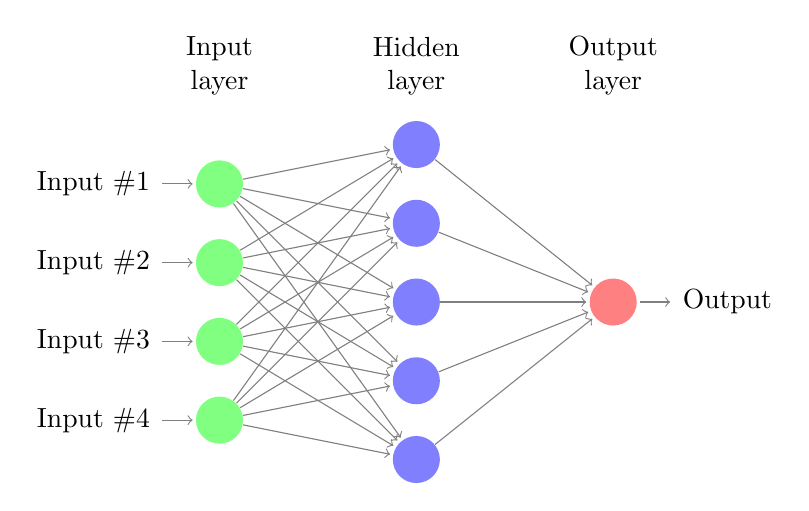
\begin{tikzpicture}[shorten >=1pt,->,draw=black!50, node distance=\layersep]
    \tikzstyle{every pin edge}=[<-,shorten <=1pt]
    \tikzstyle{neuron}=[circle,fill=black!25,minimum size=17pt,inner sep=0pt]
    \tikzstyle{input neuron}=[neuron, fill=green!50];
    \tikzstyle{output neuron}=[neuron, fill=red!50];
    \tikzstyle{hidden neuron}=[neuron, fill=blue!50];
    \tikzstyle{annot} = [text width=4em, text centered]

    % Draw the input layer nodes
    \foreach \name / \y in {1,...,4}
    % This is the same as writing \foreach \name / \y in {1/1,2/2,3/3,4/4}
        \node[input neuron, pin=left:Input \#\y] (I-\name) at (0,-\y) {};

    % Draw the hidden layer nodes
    \foreach \name / \y in {1,...,5}
        \path[yshift=0.5cm]
            node[hidden neuron] (H-\name) at (\layersep,-\y cm) {};

    % Draw the output layer node
    \node[output neuron,pin={[pin edge={->}]right:Output}, right of=H-3] (O) {};

    % Connect every node in the input layer with every node in the
    % hidden layer.
    \foreach \source in {1,...,4}
        \foreach \dest in {1,...,5}
            \path (I-\source) edge (H-\dest);

    % Connect every node in the hidden layer with the output layer
    \foreach \source in {1,...,5}
        \path (H-\source) edge (O);

    % Annotate the layers
    \node[annot,above of=H-1, node distance=1cm] (hl) {Hidden layer};
    \node[annot,left of=hl] {Input layer};
    \node[annot,right of=hl] {Output layer};
\end{tikzpicture}
\ddef{Deep Neural Network}{A neural network with multiple hidden layers is a deep neural network.}
\todo{Insert deep NN diagram}
\ddef{Deep Learning}{Deep Learning refers to the training of large neural networks.}
Neural networks were widely used in the 80s and early 90s but their popularity diminished in the late 90s. However, recent improvements in hardware and software have made neural networks state of the art again. Factors for deep learning's the recent popularity and success include:
\begin{itemize}
	\item Large quantity of data: we generate and save more data than ever before. More data generally means better NN performance.
	\item More compute power: In addition to general \href{https://en.wikipedia.org/wiki/Moore%27s_law}{Moore's Law} progress, we also have access to GPUs and distributed/cloud computing that speed up training. More compute power allows us to train bigger NNs. 
	\item Improved algorithms: Researchers continue to discover new NN architectures and algorithms that improve performance.
\end{itemize}
\section{Neural Network Basics}


\subsection{Logistic regression}
A single neuron can implement logistic regression. Let's take a look at logistic regression from a machine learning point of view by working through an example. 
\ddef{Logistic regression}{Regression model where the dependent variable (DV) is categorical. Examples: classify a tumor as either benign or malignant based on features, classify an image as either containing a hotdog or not containing a hotdog.}
Imagine we want to build a model that can determine if an image contains a cat. We have a training set of images that are labeled (i.e. we know if there is or isn't a cat in each image). If we have a 64 x 64 pixel, 3 channel image, we can turn this into a feature vector by unrolling all pixel intensity values into a long feature vector with dimensions $n_{x} = 64 \times 64 \times 3 = 12,288$.
\dbox{
IMPORTANT NOTATION

\begin{itemize}
	\item $(x, y)$ is a single training example. $x$ is a input vector and $y$ is the output variable where $x\in \mathbb{R}^{n_x}, y\in\{0, 1\}$ for binary classification.
	\item $m$ or $m_{train}$  is the number of training vectors
	\item $n_x$ or $n$ is the size of a input vector
	\item $n_y$ is the size of the output vector
	\item $(x^{(1)}, y^{(1)}, (x^{(2)}, y^{(2)}), ..., (x^{(m)}, y^{(m)})$ is the entire training set
	\item $X$ is a $(n_x \times m)$ matrix where each column is an individual training vector:
\[ X =
\begin{bmatrix}
 \vert & \vert && \vert\\
 v_1 & v_2 & \dots&  x^{(m)}\\
 \vert & \vert&& \vert
\end{bmatrix}
\]
	\item We can also stack $y$ into a $(1, m)$ matrix: $Y = \left[ \begin{matrix} y^{(1)} & Y^{(2)} & \dots & y^{(m)} \end{matrix} \right] $

\end{itemize}
}


Our implementation of logistic regression will have 3 components. The hypothesis function. The cost function measures how accurate our hypothesis is. We use the gradient descent algorithm to minimize the cost function. 

\dbox{
Hypothesis function: A function of x for fixed parameters. Given parameters $w$, function $h$ outputs a $y$ (output) value for any given $x$ (input) value.

For binary logistic regression:
Given $x$, want $\hat{y} = P(y = 1 | x)$, where $x\in \mathbb{R}^{n_x}$

Parameters: $w\in \mathbb{R}^{n_x}, b \in \mathbb{R}$

Output $\hat{y} = \sigma(w^Tx + b)$, where $\sigma(z) = \frac{1}{1 + e^{-z}}$
}

We use the sigmoid function to ensure $ 0 <= \hat{y} <= 1$.

The goal is to get $\hat{y}^{(i)} \approx y^{(i)}$

\ddef{Deep Learning}{Deep Learning refers to the training of large neural networks.}

We need a way to quantify the accuracy of our model. We need a function, $L$, that is small when $\hat{y}$ and $y$ are similar and large when $\hat{y}$ and $y$ are different. 

\dbox{Loss function: a way to measure the accuracy of a single example.

$$L (\hat{y}, y) = (1 - y)(\log(1 - \hat{y})) - (y) (\log{\hat{y}}))$$
}

Let's consider the 2 possibles values of $y$ to see how this function behaves:

When $y = 1 \implies  L (\hat{y}, 1) = (0) (\log(1 - \hat{y})) - (1) (\log{\hat{y}}) = -\log{\hat{y}}$. Then $\hat{y} = 1 \implies L(\hat{y}, 1) = 0$. The loss is 0 since $\hat{y}$ is accurate. On the other hand, $\hat{y} = 0 \implies L(\hat{y}, 1) \xrightarrow{y\to0} \infty$ so the loss is high when $\hat{y}$ is inaccurate.

When $y = 0 \implies  L (\hat{y}, 1) = (1) (\log(1 - \hat{y})) - (0) (\log{\hat{y}})  = \log(1 - \hat{y})$. Then $\hat{y} = 0 \implies L(\hat{y}, 0) = 0$ and $\hat{y} = 1 \implies L(\hat{y}, 0) \xrightarrow{y\to1} \infty$. Likewise, the loss is low when $\hat{y}$ is accurate and high when $\hat{y}$ is inaccurate.


We use the following loss function in logistic regression because it convex (smooth). Other loss functions like the square root error are non-convex in this case.

\dbox{
Cost function : a way to measure the accuracy of our hypothesis function. A function of the parameters. It is the sum of the squares of the differences between our predicted output values and the given target variables. We want to choose parameters such that our hypothesis makes reasonably accurate predictions for our training examples. The cost function is a function of the parameters $w, b$.

$$J(w, b) = \frac{1}{m}\sum_{i = 1}^{m}(L (\hat{y}, y))$$
}

The cost function is basically the average loss function over the entire training set for a given set of parameters.


\section{Shallow Neural Network}

\section{Neural Network Basics}





\section{Deep Neural Network}
